\documentclass{article}
\usepackage[utf8]{inputenc}
\usepackage[russian]{babel}
\usepackage{graphicx}
\graphicspath{ {images/} }
\usepackage{wrapfig}
\usepackage{mathtext}
\usepackage{amsmath}
\usepackage{fancyhdr}
\usepackage{wrapfig}
\usepackage{caption}
\pagestyle{fancy}
\fancyhf{}
\rhead{Труды Института механики УНЦ РАН, 2007}
\lhead{\thepage}

\begin{document}
\thispagestyle{empty}

\includegraphics[width=2cm]{label}\hfill\textbf{УДК 534.2;532}\newline\newline
\begin{center}

\fontsize{17}{10}\selectfont\textbf{Прямое численное моделированье сильного сжатия осесимметричной газовой полости в жидкости\footnote{Работа выполнена при финансовой поддержке Российского фонда фендаментальных исследований (проект № 05-01-0 0415-а) и в рамках программы ОЭММПУ РАН)}}\newline
\end{center}
\begin{center}
\fontsize{12}{10}\textit{А. А. Аганин, Т. Ф. Халитова, Н. А. Хисматуллина}
\end{center}
\begin{center}
Институт механики и машиностроения КазНЦ РАН, Казань\newline
\end{center}
\textbf{Аннотация.} 
Предлагается методика расчета сильного сжатия осесимметричного газового пузырька в жидкости методом прямого численного моделирования на основе уравенний динамики жидкости и газа. Эта методика использует схему второго порядка точности по пространству и времени в области гладких решений. Приводится результаты численного иследования экономичности данной методики. Установлено, что она намного эффективнее широко известной в литературе классической схемы Годунова первого порядка аппроксимации.
\begin{flushleft}
\textbf{Ключевые слова:}
\textsf{уравнения газовой динамики, ENO, TVD схема Годунова}
\end{flushleft}
\begin{center}
\rule{4.5cm}{0.4pt}
\end{center}
\begin{flushleft}
\section{Введение}
\end{flushleft}
При изучении эволюции возмущений сферической формы пузырька широко используется приближенные модели, в которых динамика жидкости и газа представляется как суперпозиция чисто радиального движения и его малого несферического возмущения ~\cite{litlink1}. Такой подход значительно упрощает математические выкладки и он эффективен в смысле затрат компьютерного времени. Однако точность и облать приминимости таких моделей ограничены предположениями о характере движения и распределении параметров задачи. \newline\indentВ настоящей работе предлагается методика расчета сильного сжатия осесиметричного газового пузырька в жидкости методом прямого численного моделирования на основе уравнений динамики жидкости и газа. \newline\newline Такой подход является более общим, однако требует значительных временных затрат. в связи с этим в данной работе представлены результаты численного иследования экономичности иетодики на примере тестовой задачи свободных колебаний полости в жидкости. Для иллюстрации правильности описания сферического и несфирического движения поверхности, а также их взаимодействия приводится результаты расчета задачи динамики газовой полости в слое жидкости.
\newline
\section{Математическая модель}
В настоящей работе приминяются уравнения динамики газа и сжимаемой жидкости без учета вязкости, теплопроводности и испарения-конденсации в виде:
\begin{center}
\fontsize{12}{10}{$${\frac{d p}{d t}} + {p\nabla \cdot \textbf{u}} = 0,\; {\frac{d \textbf{u}}{d t}} + {\nabla p} = 0,\; {\frac{d E}{d t}} + {\nabla \cdot p\textbf{u}} = 0$$}
\end{center}

\begin{center}
\fontsize{12}{10}{
$$\textbf{u}^{+} \cdot \textbf{n}^{o} = \textbf{u}^{-} \cdot \textbf{n}^{o} = D, \; p^+=p^- + 2H\sigma$$}
\end{center}

\begin{center}
\fontsize{12}{10}{
$$a_i(t)=\frac{2i+1}{2}\int\limits_\pi^{-\pi}r_s(\theta, t)P_i(\cos\theta)\sin\theta d\theta$$}
\end{center}

\begin{center}
 \fontsize{12}{10}{$\textbf{Q}_{\tau}+\textbf{F}_{\xi}+\textbf{G}_{\eta}=\textbf{S}, \; \textbf{q}=(\rho, \rho u,\rho\upsilon,\rho\varphi E)^{T},$}
\end{center}

\newpage
\begin{figure}[h]
\centering
\captionsetup{format=hang,justification=raggedright}
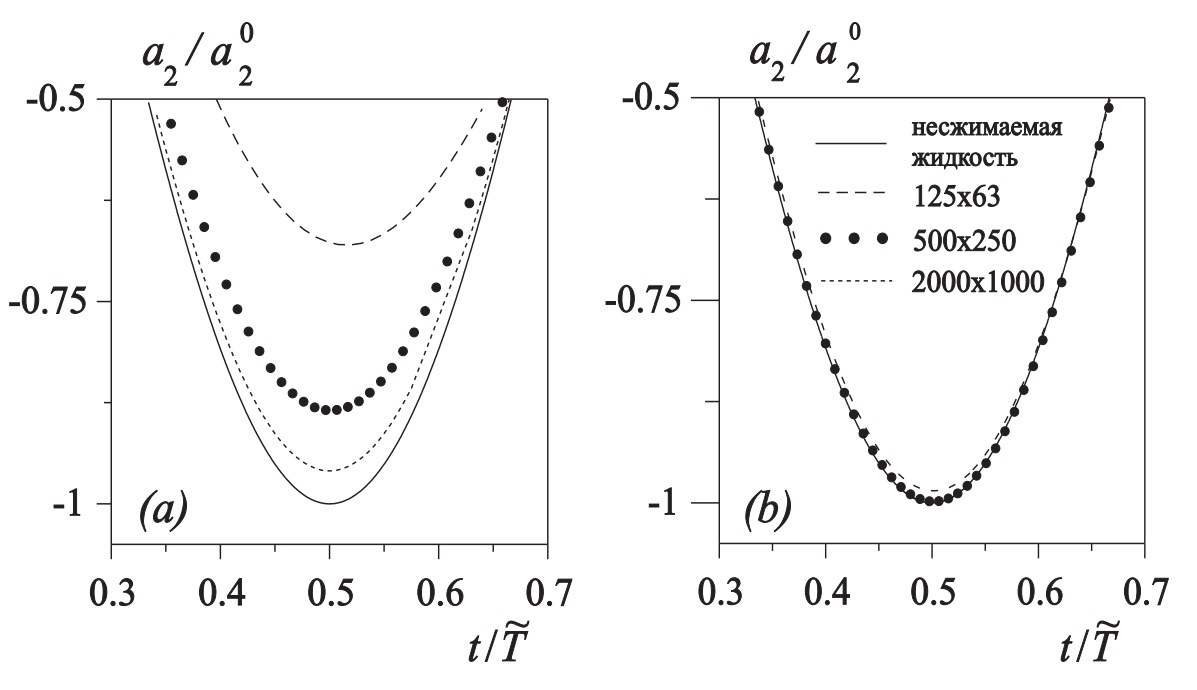
\includegraphics[scale=0.4]{pic.jpg}
\caption{Зависимость относительного отклонения от относительного времени в задаче свободный колебаний полости в жидкости при использовании a) классической схемы Годунова и b) ENO-модификации схемы Годунова на различных сетках, {$\widetilde{T}$} -  переод колебаний несжимаемой жидкости}
\end{figure}

\begin{thebibliography}{}
    \bibitem{litlink1}  Аганин А. А., Гусева Т.С. Изменение малого искажения сферической формы газового пузырька при его сильном расширении-сжатии // ПМТФ. 2005. № 4. С. 17-22.
    \bibitem{litlink2}  Годунов С. К.
\end{thebibliography}

\end{document}
